\section{Software}
\subsection{Interfaz de usuario}

Hemos desarrollado dos interfaces de usuario, una sobre una web y otra sobre una pantalla táctil.

\subsection{Interfaz web}
Para la interaccióncon el sistema, hemos diseñado un servidor web mediante el lenguaje \texttt{HTML}, estilizado mediante \texttt{CSS} y con algunas funciones creadas mediante JavaScript.

EL procesamiento de datos recibidos desde el servidor web y la creación dinámica de datos para la web se generan en diferentes archivos \texttt{CGI}, los cuales se explicarán en el \textbf{REFENCIA AL APARTADO DE LOS CGI}.

El servidor web cuenta con 4 páginas web diferentes, una principal, una para gestionar la radio, otra para gestionar el reproductor MP3 y otra para gestionar el procesado de audio. En todas estás páginas, en la esquina superior derecha, se encuentra la fecha y la hora del sistema. Todas estas páginas se explican a continuación.
\subsubsection{Configuración General}
Esta página web cuenta con una sección llamada "Camino de Audio", la cual cuenta con 4 botones que nos permiten seleccionar tanto la entrada, Radio o MP3, tanto la salida de audio, Auriculares o Altavoz.

También cuenta con una sección llamada "Bajo Consumo" que cuenta con tan solo un botón que nos permitirá poner el microcontrolador en modo bajo consumo.

Por último, cuenta con una sección llamada "Consumo", que contiene un widget que nos permite visualizar de forma dinámica en consumo medido en el sistema.

\begin{figure}[h]
    \centering
    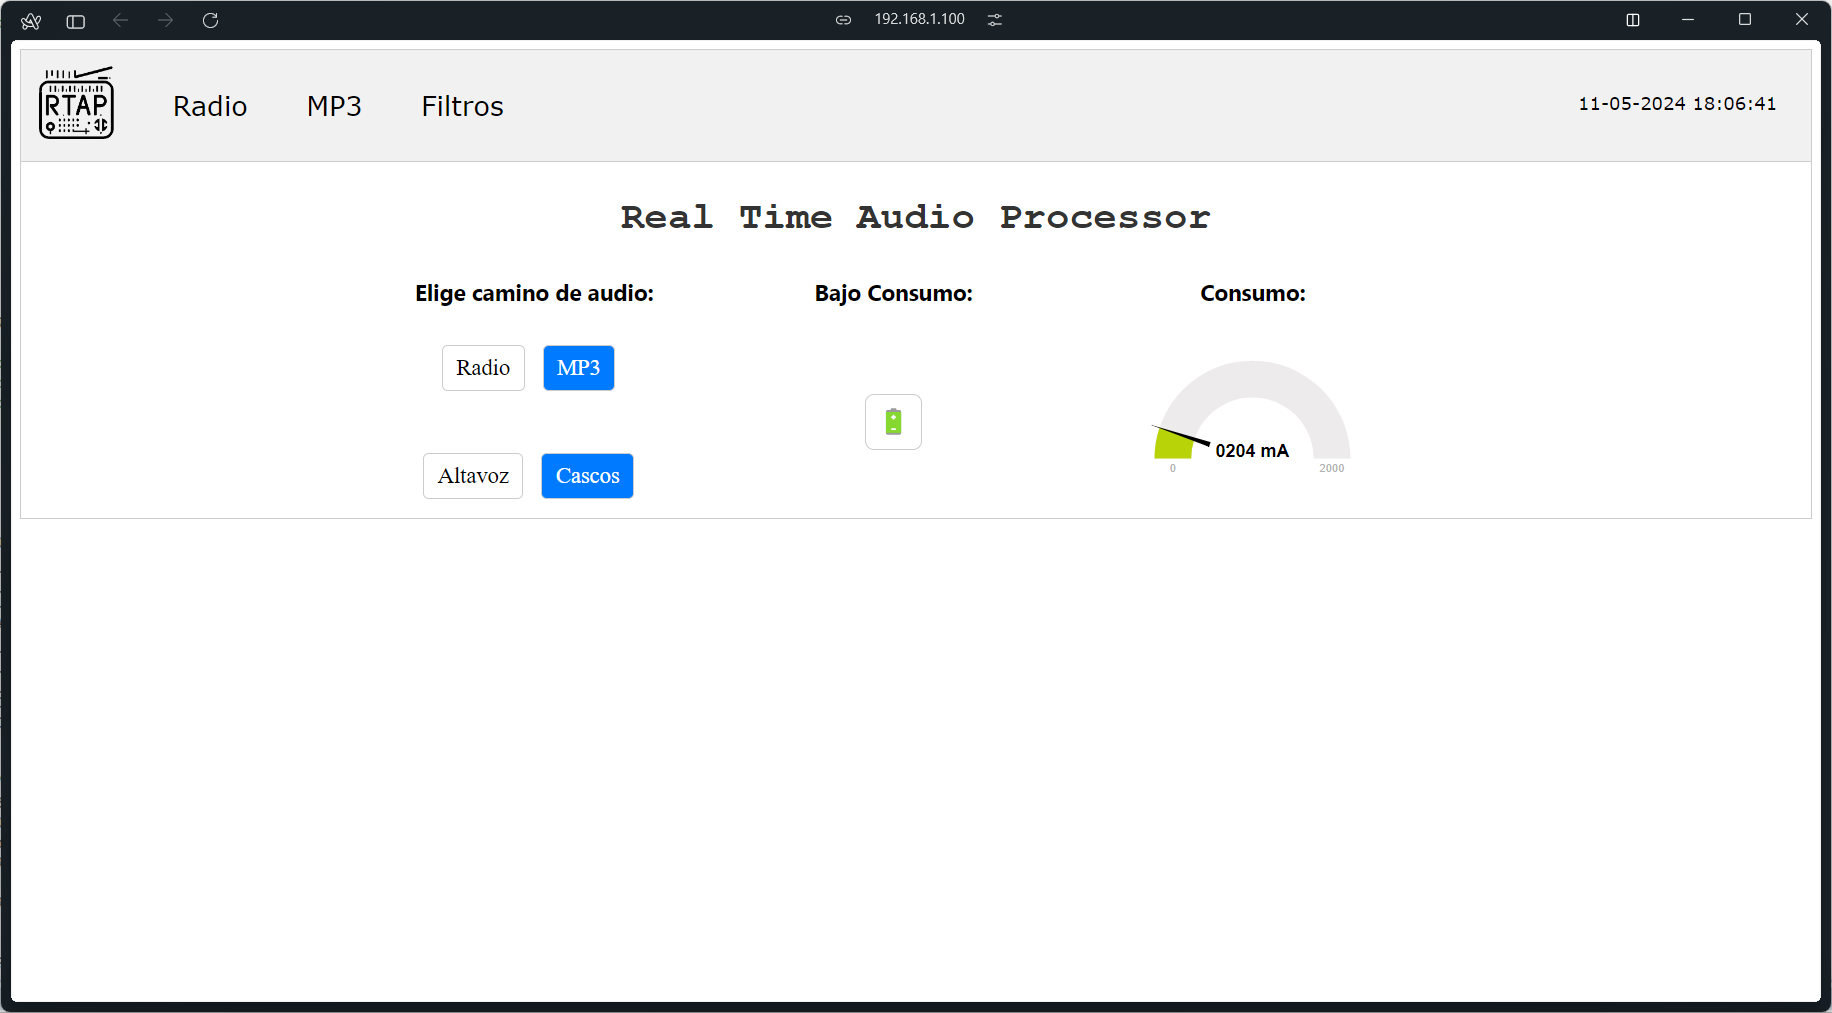
\includegraphics[width=0.6\textwidth]{images/3/3-1/3-1-1-1/Pagina_Principal.png}
    \caption{Página Principal}
    \label{fig:3-1-1-1-Principal}
\end{figure}
\subsubsection{Página Radio}
Esta página web cuenta con una primera sección llamada \textit{Sintonizar una frecuencia} la cual nos permite introducir la frecuencia que deseemos sintonizar en el recuadro blanco. Luego, mediante el botón Sintonizar, podremos sintonizar dicha frecuencia en el Sintonizador FM.

A continuación, se encuentra una sección llamada \textit{Seek}, en la cual se encuentran dos botones. El primero, que contiene una flecha hacia arriba, nos permite realizar un \textit{SeekUp}, es decir, sintonizar una frecuancia mayor con más potencia que un determinado umbral. De forma análoga, el otro botón, ilustrado mediante una flecha hacia abajo, nos permite realizar un \textit{SeekDown}, es decir, sintonizar una frecuencia menor, pero que tenga más potencia que dicho determinado umbral.

La siguiente sección llamada \textit{Volumen}, contiene un slider horizontal que nos permite selecionar el volumen de la señal de audio. También encontramos un botón de mute, es decir, situar el volumen a 0.

Por último, encontramosla sección \textit{Salida}, la cual cuenta con dos botones que nos permiten seleccionar la salida de auido deseada entre Altavoz o Auriculares.

\begin{figure}[h]
    \centering
    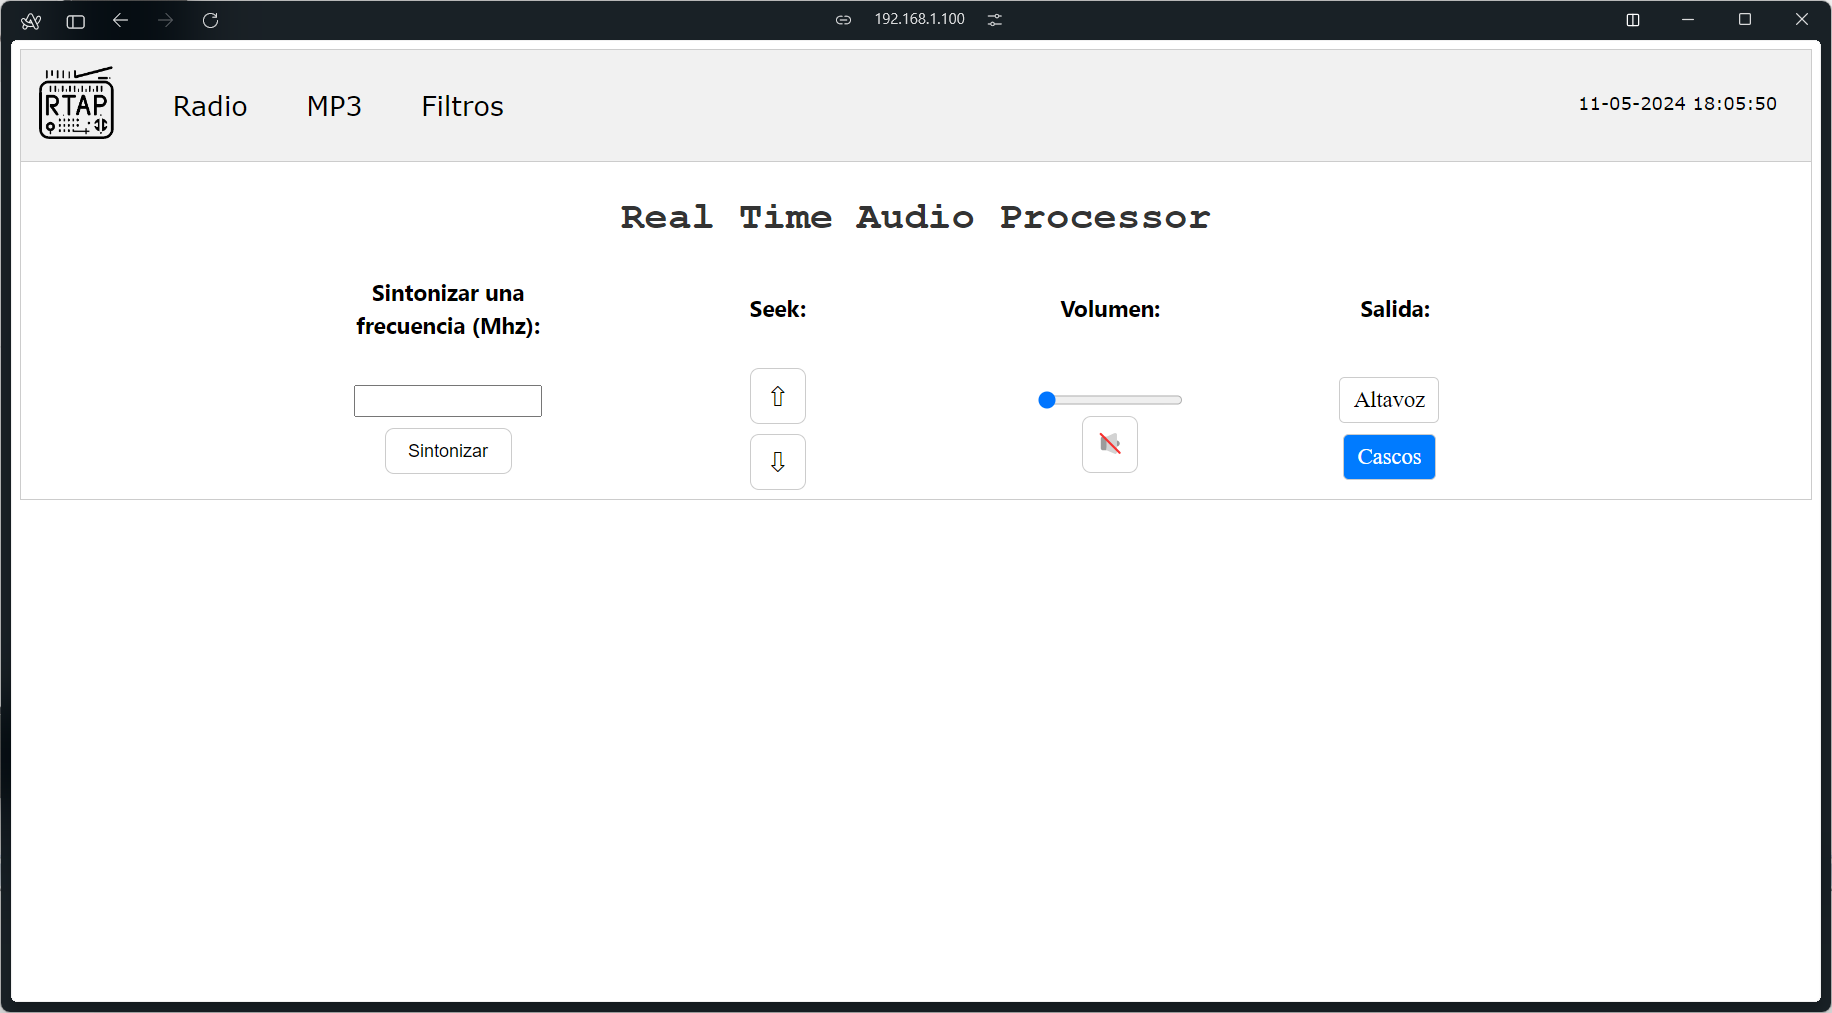
\includegraphics[width=0.8\textwidth]{images/3/3-1/3-1-1-2/Pagina_Radio.png}
    \caption{Página Radio}
    \label{fig:3-1-1-2-Radio}
\end{figure}
\paragraph{Página MP3}
En primer lugar, nos econtramos con una sección llamada \textit{Canciones}, la cual cuenta con un menú desplegable con lista, con sus correspondientes nombres, de las posibles canciones. Junto a dicho menú, se cuentra un botón que nos permite confimar la canción seleccionada.

A continuación, encontramos la sección demoninada \textit{Control} la cual cuentra con 4 botones. El primero, nos permite seleccionar la canción anterior a la canción acutal. A continuación, nos encontramos con un botón que nos permite tanto pausar como continuar la reproducción de la canción actual. El siguiente botón nos permite seleccionar la siguiente canción de la lista. Por último, el botón de abajo, nos permite activar y desactivar la puesta en bucle de la canción actual.

De forma análoga a la página de la Radio, las siguientes dos secciones nos permiten modificar el volumen del sistema y la salida de la señal de audio.

\begin{figure}[H]
    \centering
    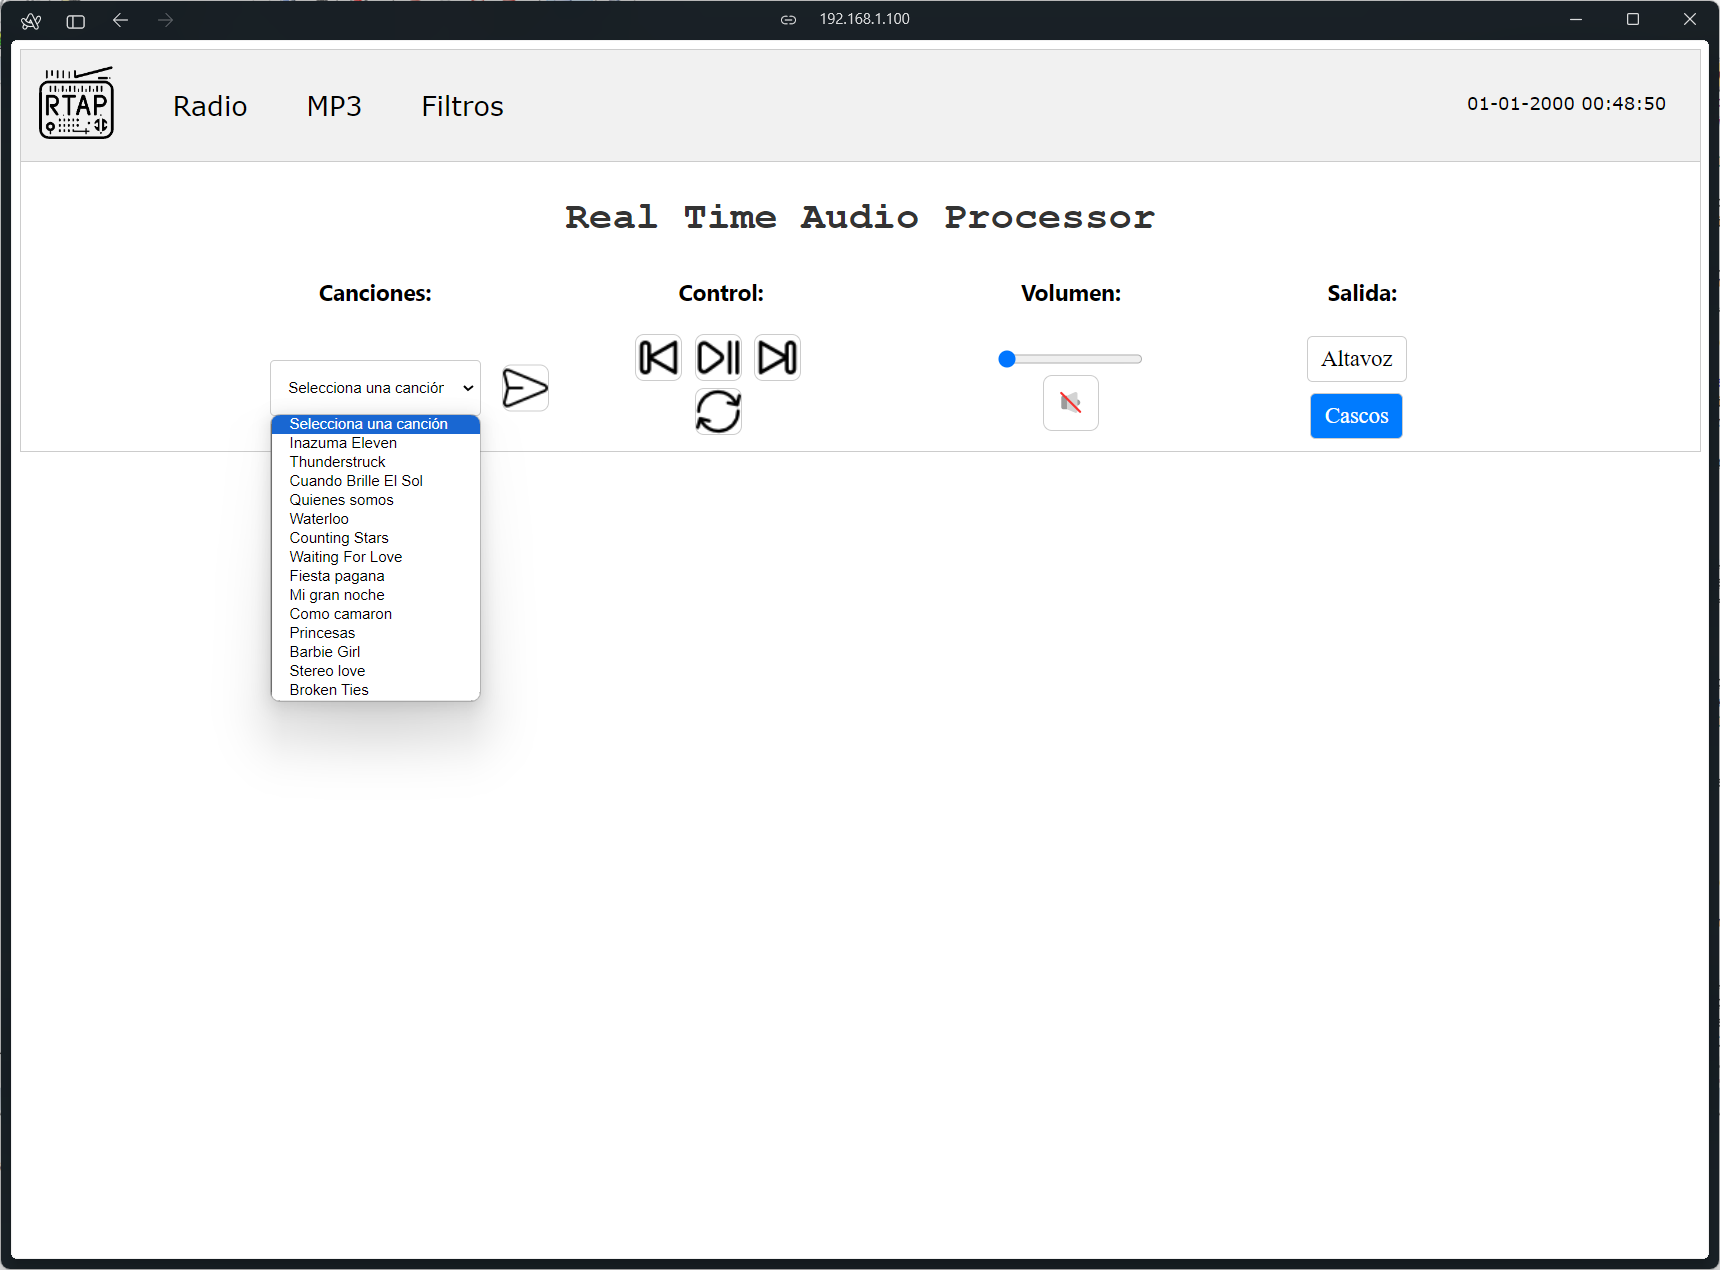
\includegraphics[width=0.8\textwidth]{images/3/3-1/3-1-1-3/Pagina_MP3.png}
    \caption{Página MP3}
    \label{fig:3-1-1-3-MP3}
\end{figure}
\subsubsection{Procesamiento de Audio}

La última página web se encarga de todo el procesamiento de audio. En primer lugar, nos encontramos con la sección llamada "Ecualizador", el cual nos permite elegir, mediante unos sliders vertiales, entre un rango de valores, la ecualización que se desee aplicar en las diferentes bandas posibles.

A continuación, en la sección denominada "Guardar Conf.", nos encontramos un botón que nos permite guardar la configuración de los distintos filtros en la tarjeta microSD conectada al sistema.

Por último, de la misma manera que en las dos anteriores páginas, nso encontramos los controles que nos permiten modificar el volumen del sistema y seleccionar la salida de auido.

\begin{figure}[h]
    \centering
    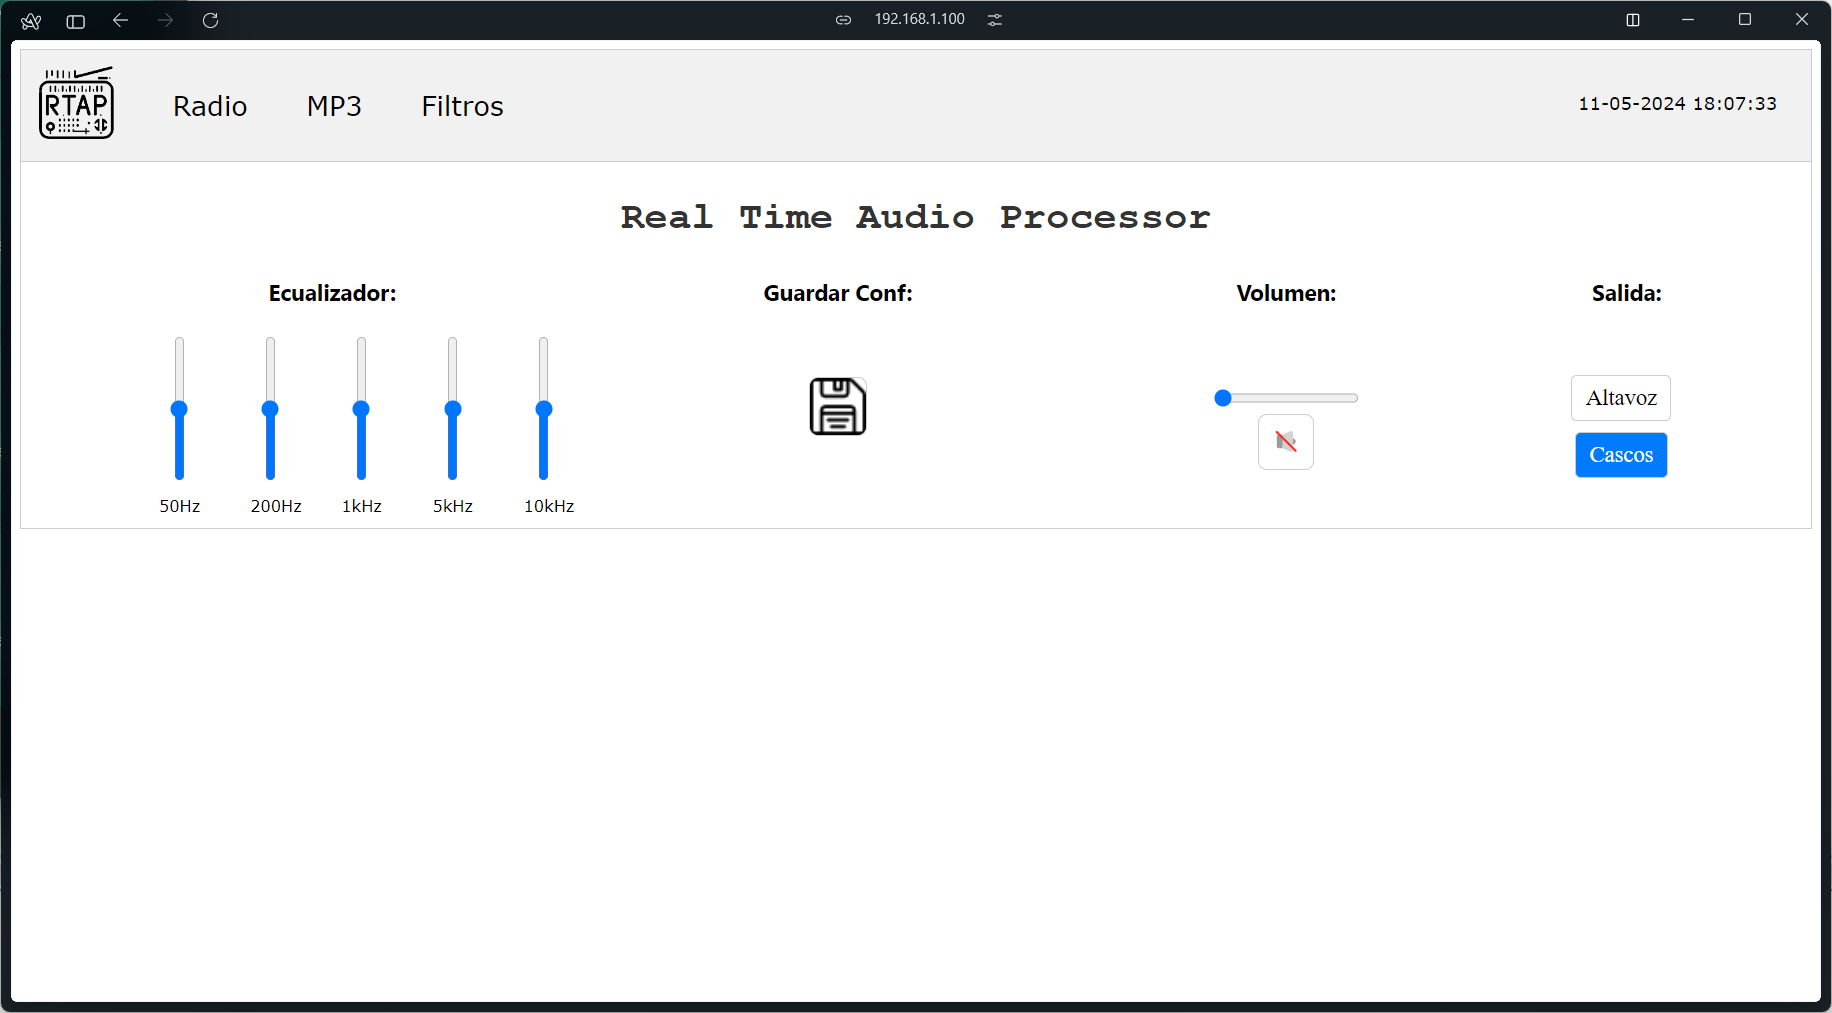
\includegraphics[width=0.6\textwidth]{images/3/3-1/3-1-1-4/Pagina_Filtros.png}
    \caption{Página Filtros}
    \label{fig:3-1-1-4-Filtros}
\end{figure}
\subsection{Interfaz táctil}

La placa STM32F769-disco que se ha utilizado en este proyecto dispone de una pantalla LCD táctil de 4.3", con una resolución de 800 x 480 píxeles y una profundidad del color de 16 bit. Esto permite crear interfaces gráficas atractivas, y, gracaias al uso de las DMA, con un coste computacional asumible. Por tanto, después de estudiar las diferentes opciones disponibles, se ha diseñado una interfaz completa, que permite el control completo del sistema.
\subsubsection{Software y librerías disponibles}
A la hora de crear una interfaz gráfica, la opción más lógica es utilizar una librería de más alto nivel, o un software de creación de interfaces, para abstraer el manejo de cada píxel individual, pero, en el mundo de los microcontroladores, estas opciones son bastante limitadas. Algunas de las opciones que se han estudiado son:
\begin{itemize}
  \item \textbf{Embedded Wizard:} Este software permite la creación de interfaces gráficas de una manera aparentemente sencilla, pero es código cerrado, y para utilizarlo de forma gratuita hay que asumir una marca de agua con su logo. Además, tienen su propio sistema operativo, que si bien no es muy distinto de las opciones conocidas, maximiza el riesgo de fallo a la hora de, por ejemplo, implementar el servidor web. Por tanto, esta opción se descartó.
  \item \textbf{EmWin:} Este software es la herramienta de Keil para la creación de interfaces, y viene incluida como \textit{software pack} dentro del programa. Incluye una función de generación de interfaces \textit{drag and drop}, lo que significa que, desde su programa, solo hay que colocar los elementos que se quieran tener en la interfaz en su sitio adecuado, todo desde una interfaz gráfica, abstrayendo el código. Sin embargo, las opciones de este software son muy limitadas, y las interfaces que genera tienen un aspecto rudimentario y obsoleto, por lo que esta opción también se descartó.
  \item \textbf{TouchGFX:} Este software, propiedad de STM, presenta una interfaz gráfica para la generación automática de código. Es un software muy potente, con el que es fácil generar interfaces modernas y visualmente atractivas. Además, incluye numerosos ejemplos, tanto en su aplicación, como en CubeMX. En un principio, se seleccionó esta opción, pero presenta el problema de ser de código cerrado, y es muy difícil adaptar el código que se genera para que sea compatible con Keil. Por tanto, finalmente se descartó.
  \item \textbf{LVGL:} Little Versatile Graphic Library es una librería de código abierto ampliamente utilizada en el mundo profesional. Varias empresas multinacionales, como Xiaomi o LG, utilizan actualmente adaptaciones de esta librería en algunos de sus productos. Es cierto que esta opción no dispone aún de herramientas para la generación automática de código, pero la librería es relativamente fácil de manejar. Con LVGL se pueden generar interfaces de todo tipo, y para el proyecto se ha seleccionado por su versatilidad y su fácil manejo. Además, ahora está presente en Keil como \textit{Software Pack}, por lo que su integración es absoluta. En nuestro proyecto, se utiliza la versión 9.1, que en el momento de redacción e implementación del proyecto, es la última versión estable de la librería.
\end{itemize}
\subsubsection{El bajo nivel}
LVGL es una librería de alto nivel, que es capaz de dibujar formas sobre un \textit{array}. Sin embargo, es responsabilidad de la persona que implementa la librería, el representar este \textit{array} en la pantalla. De este modo, el programador genera una función que representa un conjunto de píxeles en su pantalla, y LVGL se encarga de llamar a esta función cuando corresponda. Es decir, el tiempo de refresco de la pantalla variará según las necesidades del momento, liberando el uso de CPU cuando la pantalla tiene una imagen estática.

La primera aproximación posible para esta función es un simple bucle: itera todo el \textit{array} de píxeles y los envía a la pantalla. Sin embargo, esta aproximación es muy intensiva en el uso de CPU, además de poco eficiente. Por ello, una vez se ha determinado que el funcionamiento de la pantalla y el de LVGL es correcto, conviene modificarla. En el caso de RTAP, esta función utiliza la DMA 2, el \textit{Stream} 2 y el Canal 2, en configuración \textit{Memory To Memory}, consiguiendo alcanzar la tasa de refresco máxima que soporta la pantalla, de 30 fps, con un uso de la CPU mínimo, excepto cuando se ejecutan animaciones, que el uso de CPU aumenta considerablemente.

Una de las razones por las que la tasa de refresco disminuye es por el modo de funcionamiento de LVGL: admite diferentes configuraciones de \textit{buffer} que pasará como parámetro a la función de bajo nivel. En nuestro proyecto se utilizan de manera simultánea dos \textit{buffers} (la pantalla lee de uno mientras el controlador escribe en otro, y luego conmutan), pero cada uno solamente es del tamaño de la décima parte de la pantalla. Gracias a esta configuración es posible ahorrar mucha memoria, a cambio de un mayor uso de la CPU.

\subsubsection{El alto nivel}
Una vez se ha configurado una función de bajo nivel para representar los píxeles en la pantalla, se pueden utilizar las abstracciones de alto nivel que ofrece LVGL. 

La interfaz gráfica de RTAP consta de 4 pestañas: Inicio, Radio, MP3 y Filtros. A su vez, cada pestaña dispone de un lienzo en color gris claro, sobre el que se añaden paneles, con un fondo blanco y un borde gris de 2 píxeles de grosor. Cada panel implementa una funcionalidad, o muestra la información relevante. Todas las pestañas comparten una filosofía: Los paneles principales ocupan la totalidad de la pantalla, haciendo la interfaz muy intuitiva, y, si se desliza el panel hacia la parte superior, se muestran los créditos del proyecto: El título, la asignatura y los estudiantes involucrados. Además, todo el proyecto utiliza la fuente \textit{Montserrat}, variando el tamaño según la importancia del contenido. A continuación, se explica cada una de las pestañas, excluyendo el panel de créditos. 

\textbf{Inicio}

La pestaña de inicio consta de dos paneles principales: Configuración rápida y Consumo.
\begin{itemize}
    \item \textbf{Configuración rápida:} Este panel está formado por tres grupos de botones. El primer y el segundo grupo se emplean para seleccionar la salida y la entrada, respectivamente. Como el sistema no permite la opción de seleccionar las dos entradas o las dos salidas simultáneamente, estos botones son excluyentes: marcar uno desmarca el otro. Como estilo, se ha optado por un color azul claro para representar la opción seleccionada, y un color más oscuro para la no seleccionada. Por último, este panel tiene un botón que hace que el sistema entre en modo de bajo consumo. Los botones se distribuyen según una rejilla fija, y los grupos de estos se dividen mediante un espaciado uniforme, calculado de manera dinámica por LVGL.
    \item \textbf{Consumo:} Este panel está formado por una escala en forma de arco, que ocupa 225º de la circunferencia. Además, se le aplica una rotación de 180º para conseguir la posición deseada, que deja espacio suficiente para colocar una etiqueta de texto. 
    
    La escala, que se utiliza para representar de forma gráfica el consumo del sistema, admite valores entre 0 y 1500, que se interpretan como miliamperios. A la escala se le aplican tres formatos diferentes: El primero es un color verde, para los valores entre 0 y 375, el segundo, un color azul, entre 375 y 1125, y el tercero, en rojo, para los valores más altos, entre 1125 y 1500. En total, la escala cuenta con 25 \textit{ticks}, y cada 4 de estos, se introduce uno principal, es decir, para los valores más significativos, de 0 A, 0.25 A, 0.5 A, 0.75 A, 1 A , 1.25 A y 1.5 A. Estos \textit{ticks} principales tienen un grosor de 2 píxeles, mientras que los secundarios tienen un grosor de 1 píxel. LVGL calcula la longitud de cada \textit{tick} de manera dinámica. Por último, la escala cuenta con una aguja, en color rojo y con una longitud máxima de 80 píxeles, que apunta al valor del consumo instantáneo, que además se representa en la etiqueta de texto.

    El panel se organiza según una rejilla flexible organizada en forma de columna. Esto significa que simplemente se declaran los objetos y se les da un tamaño, y LVGL los coloca de forma dinámica apilados verticalmente. Sin embargo, para conseguir que la etiqueta se muestre en el lugar apropiado, se le da una posición fija relativa al panel.
\end{itemize}

\textbf{Radio}

La pestaña de radio está formada por tres paneles principales: Uno para la radio, otro para el volumen, y otro para la salida.

\begin{itemize}
    \item \textbf{Radio:} Este panel es el más grande de esta pestaña, ocupando dos terceras partes del espacio. Este panel es muy complejo, estando formado por una superposición de elementos. De manera simple: En la parte posterior encontramos un título, que indica que el panel es para sintonizar una frecuencia. En la posición inmediatamente inferior, se muestra un número, que en caso de no tener ningún valor, se mostrará en color sombreado. Hay varias formas de modificar este valor, que se detallan más adelante. Después encontramos una escala, que simula la apariencia de una radio clásica, y cuyos valores, entre 87 y 108, se interpretan como megahercios. Sin embargo, en un primer plano, encima de la escala, encontramos un slider, del cual solo se representa el mando, en color rojo y con un borde negro. En LVGL un slider solo puede tener valores enteros, por lo que este toma valores entre 870 y 1080, para mantener un decimal, interpretándose el valor como centenas de kilohercio. En la parte inferior hay un espacio en blanco, cuya utilidad se comenta a continuación, y después hay una fila con un objeto en forma de caja, inicialmente vacío, y a su derecha, tres botones.

    Empezando por el slider, que puede ser la opción más intuitiva, un deslizamiento sobre la escala tendrá diferentes consecuencias: El texto que tiene encima se modificará, acompañando el valor del texto, y, en caso de ser una cadena conocida, en el espacio en blanco que se mencionó anteriormente, se representará el texto correspondiente al nombre de la cadena. Sin embargo, para no saturar la cola de mensajes ni a la radio, la cadena marcada sólo se sintoniza una vez se ha soltado el slider.

    Otra posible forma de modificar el valor de la frecuencia es mediante los botones de \textit{Seek}. El sistema busca la siguiente cadena con una señal aceptable, la sintoniza, y modifica el valor del texto y del slider. Otra opción es tocar el valor del texto, y se desplegará un teclado numérico, que permite sintonizar de manera rápida y precisa una cadena, solo en caso de haber introducido un valor correcto. En caso de que el valor introducido no sea un valor posible, o sea un número mal formado, el slider se truncará hacia el valor correcto más próximo. Para cerrar el teclado, se puede utilizar cualquiera de los dos botones pensados para ello, o tocar en cualquier parte de la pantalla.

    Además, se dispone de un botón de favoritos, que almacenará en la caja todas las cadenas que se quieran guardar (no es persistente). En caso de que se conozca el nombre de la cadena, será esto lo que se muestre en la lista, en caso contrario, se mostrará únicamente la frecuencia. Para recuperar cualquier cadena guardada, solo habrá que buscarla en la lista.

    Por último, destacar que cualquier cambio en la web se verá reflejado de forma inmediata en el slider y en todos los cuadros de texto.
    \item \textbf{Volumen:} Este panel permite ajustar el volumen global del sistema. Se mantiene sincronizado con los paneles de volumen de otras pestañas, y presenta un botón de mute, que ejecuta una animación, variando el valor hasta 0 de forma suave, o, en caso de estar ya en cero, aumentándolo hasta la posición previa. Igual que con otros sliders, para no saturar los mecanismos de sincronización, el valor solo es enviado una vez se ha soltado.
    \item \textbf{Salida:} Este panel también permite seleccionar la salida del sistema. Se mantiene sincronizado con los botones que ofrecen la misma función en otras pestañas, y mantiene el mismo estilo que el de la pestaña de inicio para indicar cuál es la opción seleccionada.
\end{itemize}

\textbf{MP3}

La pestaña del MP3 mantiene muchas similitudes con la de la radio: Se compone de tres paneles, de los cuales el principal también ocupa dos tercios de la pantalla, y los dos paneles de su derecha son idénticos a los explicados anteriormente. 

El panel principal del MP3 también es un panel muy complejo. En este caso, el panel a su vez está compuesto por varios paneles. En un primer momento, se aprecian los 3 botones principales del MP3: anterior, play/pause y siguiente. El color de estos botones se ha pensado para romper con la monotonía del sistema, dando una impresión más alegre. El degradado se calcula automáticamente por LVGL, no se aplica ninguna textura que ocupe memoria.

En la parte inferior del panel hay una pestaña, que si se desliza hacia arriba, pasa a ocupar el 70\% del subpanel. Sin embargo, a los botones se les permite ocupar el 40\% del panel, con esto se logra la impresión de que los botones no terminan de esconderse nunca. Esta pestaña representa la lista de canciones que se tiene almacenada en la tarjeta SD. Al hacer click sobre una canción, esta se envía al MP3, y además, se reproduce una animación, que sustituye durante unos segundos al título de la pestaña, representando la canción. Nuevamente, si se oculta la lista de canciones, los botones de control pasan a ocupar el 100\% de su panel.

\textbf{Filtros}

La pestaña correspondiente a los filtros muestra las opciones de ecualización del sistema, además de algunos ajustes para el audio. En concreto, esta pestaña consta de 4 paneles: 
\begin{itemize}
    \item \textbf{Ecualizador:} Es el panel principal de la pestaña, y ocupa la mitad de esta. Se compone de 5 sliders, que manejan cada uno una banda. Como en sliders anteriores, el valor únicamente se envía cuando se libera el slider. Modificar un valor en la página web ejecuta una animación para sincronizar el valor.
    \item \textbf{Volumen:} Tiene un tamaño ligeramente inferior al de las pestañas anteriores, pero mantiene el mismo valor y funcionalidad.
    \item \textbf{Guardar config:} Es un pequeño panel con un único botón, para almacenar la configuración.
    \item \textbf{Configuración de audio:} Es parecido al panel de configuración rápida de la pestaña de inicio, manteniendo el estilo y todos los botones, excepto el de bajo consumo, que en este caso es reemplazado por un botón para restablecer el valor de los filtros. Pulsar el botón hace que se ejecuten 5 animaciones, una para cada slider, poniendo su valor a cero de forma suave.
\end{itemize}

\subsubsection{Consideraciones sobre LVGL}

Después de haber repasado de forma general la interfaz del proyecto, se entiende que para representar un sistema tan complejo hace falta una cantidad considerable de memoria. En concreto, se asignan 81072 bytes de memoria a LVGL, y un stack de 7400 bytes al hilo que gestiona el funcionamiento de LVGL.

\subsection{Módulos software}

Para la implementación software se han diseñado módulos independientes para cada tarea, implementando casi todos como un hilo (o tarea) del sistema operativo de tiempo real de Keil, utilizado a través de la API CMSIS RTOS2.

Para la comunicación entre hilos hemos utilizado principalmente colas de mensajes al ser la opción más cómoda y sencilla de implementar, aunque hay un par de candados de exclusión mutua (\texttt{mutex}) y alguna \textit{flag} de hilo.

\subsubsection{Módulo de control}

El módulo de control es el encargado de orquestar la aplicación. Para incrementar el rendimiento, se ha decidido modelar con una arquitectura basada en eventos, por lo que el módulo se encuentra permanentemente esperando en una cola y sólamente reacciona cuando le llega un mensaje por ella, volviendo a esperar al finalizar la respuesta.

Para evitar tener que realizar una estructura de polling de colas, en la que el hilo debe comprobar constantemente varias colas, se ha implementado una estructura unificada de mensajes de entrada al módulo de control, de forma que solo se tiene que esperar a una sola cola. Además, cuenta con acceso a las colas de entrada de todos los demás módulos, en las que introduce mensajes como reacción a los eventos que ocurran.

Se podría realizar una estructura que contuviera todos los posibles parámetros de mensajes y un identificador para saber cuales son los útiles, pero esto es muy poco óptimo en memoria y puede tener un gran impacto en el rendimiento de la aplicación. Por ello, hemos decidido implementar una estructura basada en uniones con un campo que identifica cual es la forma de dicha unión. 

\begin{lstlisting}[captionpos=t, caption={Estructura para los mensajes al control}]
    /**
    * @brief Enumeracion de los tipos de mensaje de entrada al modulo de control
    */
   typedef enum {
       MSG_NFC,   /**< Lectura de una tarjeta del NFC */
       MSG_LCD,   /**< Mensaje de entrada del LCD     */
       MSG_WEB,   /**< Mensaje de entrada de la web   */
       MSG_RTC,   /**< Mensaje de entrada del RTC     */
       MSG_CONS,  /**< Mensaje de entrada del consumo */
       MSG_RADIO, /**< Mensaje de entrada de la radio */
   } msg_ctrl_type_t;

    /**
    * @brief Estructura para los mensajes de entrada
    */
    typedef struct {
        msg_ctrl_type_t type;    /**< Tipo de mensaje de entrada. 
                                    Dependiendo de este valor se debe interpretar el contenido */
        union {
            nfc_msg_t nfc_msg;   /**< Contenido de un mensaje de tipo MSG_NFC   */
            lcd_msg_t lcd_msg;   /**< Contenido de un mensaje de tipo MSG_LCD   */
            rtc_msg_t rtc_msg;   /**< Contenido de un mensaje de tipo MSG_RTC   */
            web_msg_t web_msg;   /**< Contenido de un mensaje de tipo MSG_WEB   */
            uint16_t  cons_msg;  /**< Contenido de un mensaje de tipo MSG_CONS  */
            uint32_t  radio_msg; /**< Contenido de un mensaje de tipo MSG_RADIO */
        };
    } msg_ctrl_t;
\end{lstlisting}

Como se puede ver, dependiendo del valor del campo \texttt{type}, tenemos un contenido u otro. Esto permite reducir significativamente la estructura pero requiere de una comprobación de qué tipo de mensaje es antes de acceder a los campos, ya que si no se podrían malinterpretar los mensajes. Se puede ver el contenido de cada tipo de mensaje en el código del \autoref{anexo:mensajes-control}.

Este módulo actua como una inteligencia central de redirección de eventos. A excepción de los GPIO de selección de canal, el módulo únicamente redirige eventos de un módulo a otros, realizando una conversión de datos en los casos que es necesaria.

Por ejemplo, cuando alguien cambia una banda del ecualizador en la pantalla táctil, este módulo recibe un mensaje de tipo \texttt{MSG\_LCD}, por lo que interpreta su contenido como un \texttt{lcd\_msg}, que a su vez contiene un campo de subtipo de mensaje y una carga útil. En este ejemplo, el subtipo sería \texttt{LCD\_BANDS} y la carga útil, de dos bytes, contendría la banda seleccionada y la amplitud que se ha cambiado. Entonces, el módulo principal interpretaría este mensaje y realizaría las dos acciones pertinentes: Enviar un mensaje de tipo \texttt{WEB\_OUT\_BANDS} a la web para que se actualice la información y otro al módulo de procesado digital para que reconfiguren los filtros. Una vez finalizado, se volvería a esperar al siguiente mensaje de la cola.

En tiempo de arranque, este módulo se encarga de habilitar el circuito de audio, enciende la radio y el MP3. Además, utiliza el módulo de la SD para leer la configuración almacenada en los ficheros y configurar tanto la lista de canciones como los filtros.

Además, este módulo es el encargado de poner el sistema en modo bajo consumo. Al entrar en modo bajo consumo, bien por la web o por la pantalla táctil, se realiza el siguiente procedimiento:
\begin{enumerate}
    \item Apagar la radio y el MP3 
    \item Deshabilitar el circuito de alimentación
    \item Limpiar las flags del procesador de \textit{Wakeup}
    \item Desactivar el \textit{Wakeup} a través del RTC y sus alarmas
    \item Entrar en modo Standby
\end{enumerate}

Hemos decidio utilizar el modo standby ya que nuestro sistema no necesita mantener ninguna información en memoria dinámica durante la ejecución del sistema. En este modo, se desactivan los periféricos y el procesador, quedando únicamente a la espera de una señal de \textit{Wakeup} para volver a despertarse. Como dicha señal hemos decidido utilizar el botón azul de la placa, ya que está conectado a un puerto con dicha capacidad.

Como el sistema se desactiva por completo y se pierde el contenido de la memoria, el sistema vuelve a partir desde cero, como si se acabara de conectar la alimentación. Esto es un comportamiento favorable, ya que se vuelven a configurar todos los pines, periféricos y direcciones de memoria adecuadamente y permite un menor consumo que los modos \textit{Sleep} o \textit{Stop}.

Otro factor destacable es que toda la configuración de este módulo en cuanto a pines y niveles lógicos, así como la configuración del módulo de medición de consumo se puede ajustar en el fichero \texttt{controlConfig.h}, permitiendo una reconfiguración rápida de ambos módulos.
\subsubsection{Módulo de control de consumo}

El módulo de medición de consumo se encarga simplemente de realizar medidas periódicas y enviarlas al módulo de control.

Dicho módulo utiliza el \texttt{ADC3} de la placa para medir el consumo que reporta el módulo analógico de consumo (\autoref{subsubsec:medidor-consumo-analog}). Dicho módulo reporta la corriente con una ganancia de $1.1 V/A$, que junto a la resolución del \texttt{ADC} de 12 bits para $3.3\ V$, ofrece una resolución efectiva de:
\[
    S_{cons} = \frac{S_{ADC}}{S_{med}} = \frac{\frac{3.3\ V}{2^{12}}}{1.1\ V/A} = 244.14\ \mu A
\]

Para nuestra aplicación, es una precisión más que suficiente.

El hilo arranca la medida del \texttt{ADC}, realiza una espera para dejar tiempo a que se complete, lee el contenido y lo envía a la cola del sistema operativo, volviendo al principio del proceso.
\subsubsection{Módulo de acceso concurrente al I2C}\label{subsec:i2c}

La placa \texttt{STM32F769NI-DISCO} ofrece únicamente un bus \texttt{I2C} en sus pines de extensión, por lo que nos vemos obligados a utilizarlo para tanto la radio como el NFC. Por tanto, hemos creado un módulo de protección para el acceso concurrente a este periférico. 

Dicho módulo únicamente utiliza un candado de exclusión mutua (\texttt{Mutex}) para evitar que ambos módulos intenten acceder a dicho periférico. Hemos creado una interfaz homónima con CMSIS Driver para que no sea necesario modificar el código existente en demasiada medida.

La principal dificultad del diseño de este módulo es la necesidad de cambiar el hilo al que se avisa en la \textit{callback} del periférico \texttt{I2C}, que se llama desde la interrupción cuando ha finalizado la transferencia. Para solucionarlo, hemos tenido que utilizar una variable estática que contiene el identificador del hilo que esta actualmente utilizando el periférico, obtenido mediante la función \texttt{osThreadGetId} que ofrece el sistema operativo.

Por tanto, el proceso de las funciones de envío y recepción de información es:
\begin{enumerate}
    \item Cerrar el candado (\texttt{osMutexAcquire})
    \item Colocar el ID del hilo actual en la variable estática
    \item Llamar a la función homónima de CMSIS Driver
    \item Esperar a la flag \texttt{FLAGS\_I2C\_DONE} que se envía cuando finaliza la transferencia
    \item Liberar el candado (\texttt{osMutexRelease})
\end{enumerate}

Con este proceso conseguimos evitar una colisión en el acceso al periférico y las posibles condiciones de carrera que conllevaría. Al ser comunicación \texttt{I2C}, no hay problema de que se alternen la comunicación entre los dos módulos ya que los esclavos ignoran los paquetes que no son para ellos.

\subsubsection{Módulo de procesado digital}

El módulo de procesado digital es el encargado de tomar las muestras, procesarlas y generar la señal de salida. Se utiliza un \texttt{ADC} de la placa para tomar muestras a $48\ kHz$ y un \texttt{DAC} para la generación de la salida, a la misma velocidad.

\paragraph{Temporización}

La temporización de este módulo es crítica, ya que es la que garantiza la calidad de la señal procesada. 

Se utiliza un \textit{Timer} de la placa, concretamente el \texttt{TIM2} para la generación de dicha señal. Para ello, el \textit{Timer} cuenta con una señal específica de sincronización para disparar eventos de conversión, \texttt{TRGO2}. Para habilitarla, se necesita además configurar el \textit{timer} como \textit{master}, como se puede ver en el \autoref{lst:conf-tim2}.

\begin{lstlisting}[captionpos=t, caption={Configuración del \textit{timer} de sincronización}]
    int dsp_tim_init(void) {
        __DSP_TIM_ENABLE();
        htim.Instance = DSP_TIM_INSTANCE;

        htim.Init.Prescaler = DSP_TIM_PRESCALER;
        htim.Init.Period = DSP_TIM_PERIOD;

        if (HAL_TIM_Base_Init(&htim)) {
            return -1;
        }

        TIM_ClockConfigTypeDef sClockConfig = {.ClockSource = TIM_CLOCKSOURCE_INTERNAL};
        if (HAL_TIM_ConfigClockSource(&htim, &sClockConfig)) {
            return -1;
        }

        TIM_MasterConfigTypeDef sMasterConfig = {
            .MasterOutputTrigger = TIM_TRGO_UPDATE,
            .MasterSlaveMode = TIM_MASTERSLAVEMODE_DISABLE,
        };
        if (HAL_TIMEx_MasterConfigSynchronization(&htim, &sMasterConfig)) {
            return -1;
        }

        if (HAL_TIM_Base_Start(&htim)) {
            return -1;
        }

        return 0;
    }
\end{lstlisting}

Una vez configurado este timer, habrá que configurar al \texttt{ADC} y al \texttt{DAC} para que realicen las conversiones disparados por dicha señal, como se verá en los siguientes apartados.

\paragraph{Adquisición de audio}

La adquisición de audio, como ya se ha comentado, se realiza a través de un \texttt{ADC}. Este se configura con los siguientes parámetros:
\begin{enumerate}
    \item Adquisición a través del \texttt{GPIO A6}
\end{enumerate}
\subsubsection{Módulo NFC}

Permite que se seleccionen canciones y emisoras mediante el móvil con NFC.


Los ficheros más destacables del módulo son:

\begin{enumerate}
	\item \texttt{nfc.c}: Hilo que gestiona el uso de la tag. Los datos obtenidos se envían por una cola al hilo de control.
	\item \texttt{nfc.h}: Exporta la función para el arranque del hilo.
\end{enumerate}

El principal problema a la hora de utilizar este componente, es que no pueden estar activos al mismo tiempo, por lo que hemos tenido que adaptar la utilización de estos dos protocolos con el uso real de nuestro módulo NFC. A la hora de guardar y leer datos, en ambos casos, se guardan en NDEF. 

Nosotros vamos a utilizar RF mediante el uso del teléfono móvil para escribir en el NDEF, mientras que el I2C para leer el contenido, por lo que solo contaremos con esos uso. Para escribir mediante RF, la tranferencia consiste en dos pulsos a nivel bajo en el GPO. 

Por esto mismo, el código consiste en habilitar el RF (DIS = 0), esperar a una subida en el GPO y esperar 500 ms (Asegurando que se ha completado la transferencia). Después, se deshabilita el RF (DIS = 1) y se procede a enviar todas las transmisiones por I2C. Finalmente, se envía la información al hilo de control y se procede a habilitar de nuevo el RF y volver a esperar al flanco de subida.

A la hora de trabajar con el I2C, utilizaremos la familia de comandos NFC Forum Type 4 Tag, mientras que con RF se utiliza ISO/IEC 7816-4. En lo referente a I2C, tenemos que crear las tramas correspondientes a cada comando. Nosotros utilizaremos:

\begin{enumerate}
\item NDEF Tag Application Select: Selecciona la aplicación NDEF Tag.
\item NDEF Select: Selecciona el fichero NDEF.
\item Read Binary: Lee datos de un fichero.
\end{enumerate}

Los utilizaremos de la siguiente manera:

\begin{figure}[h]
    \centering
    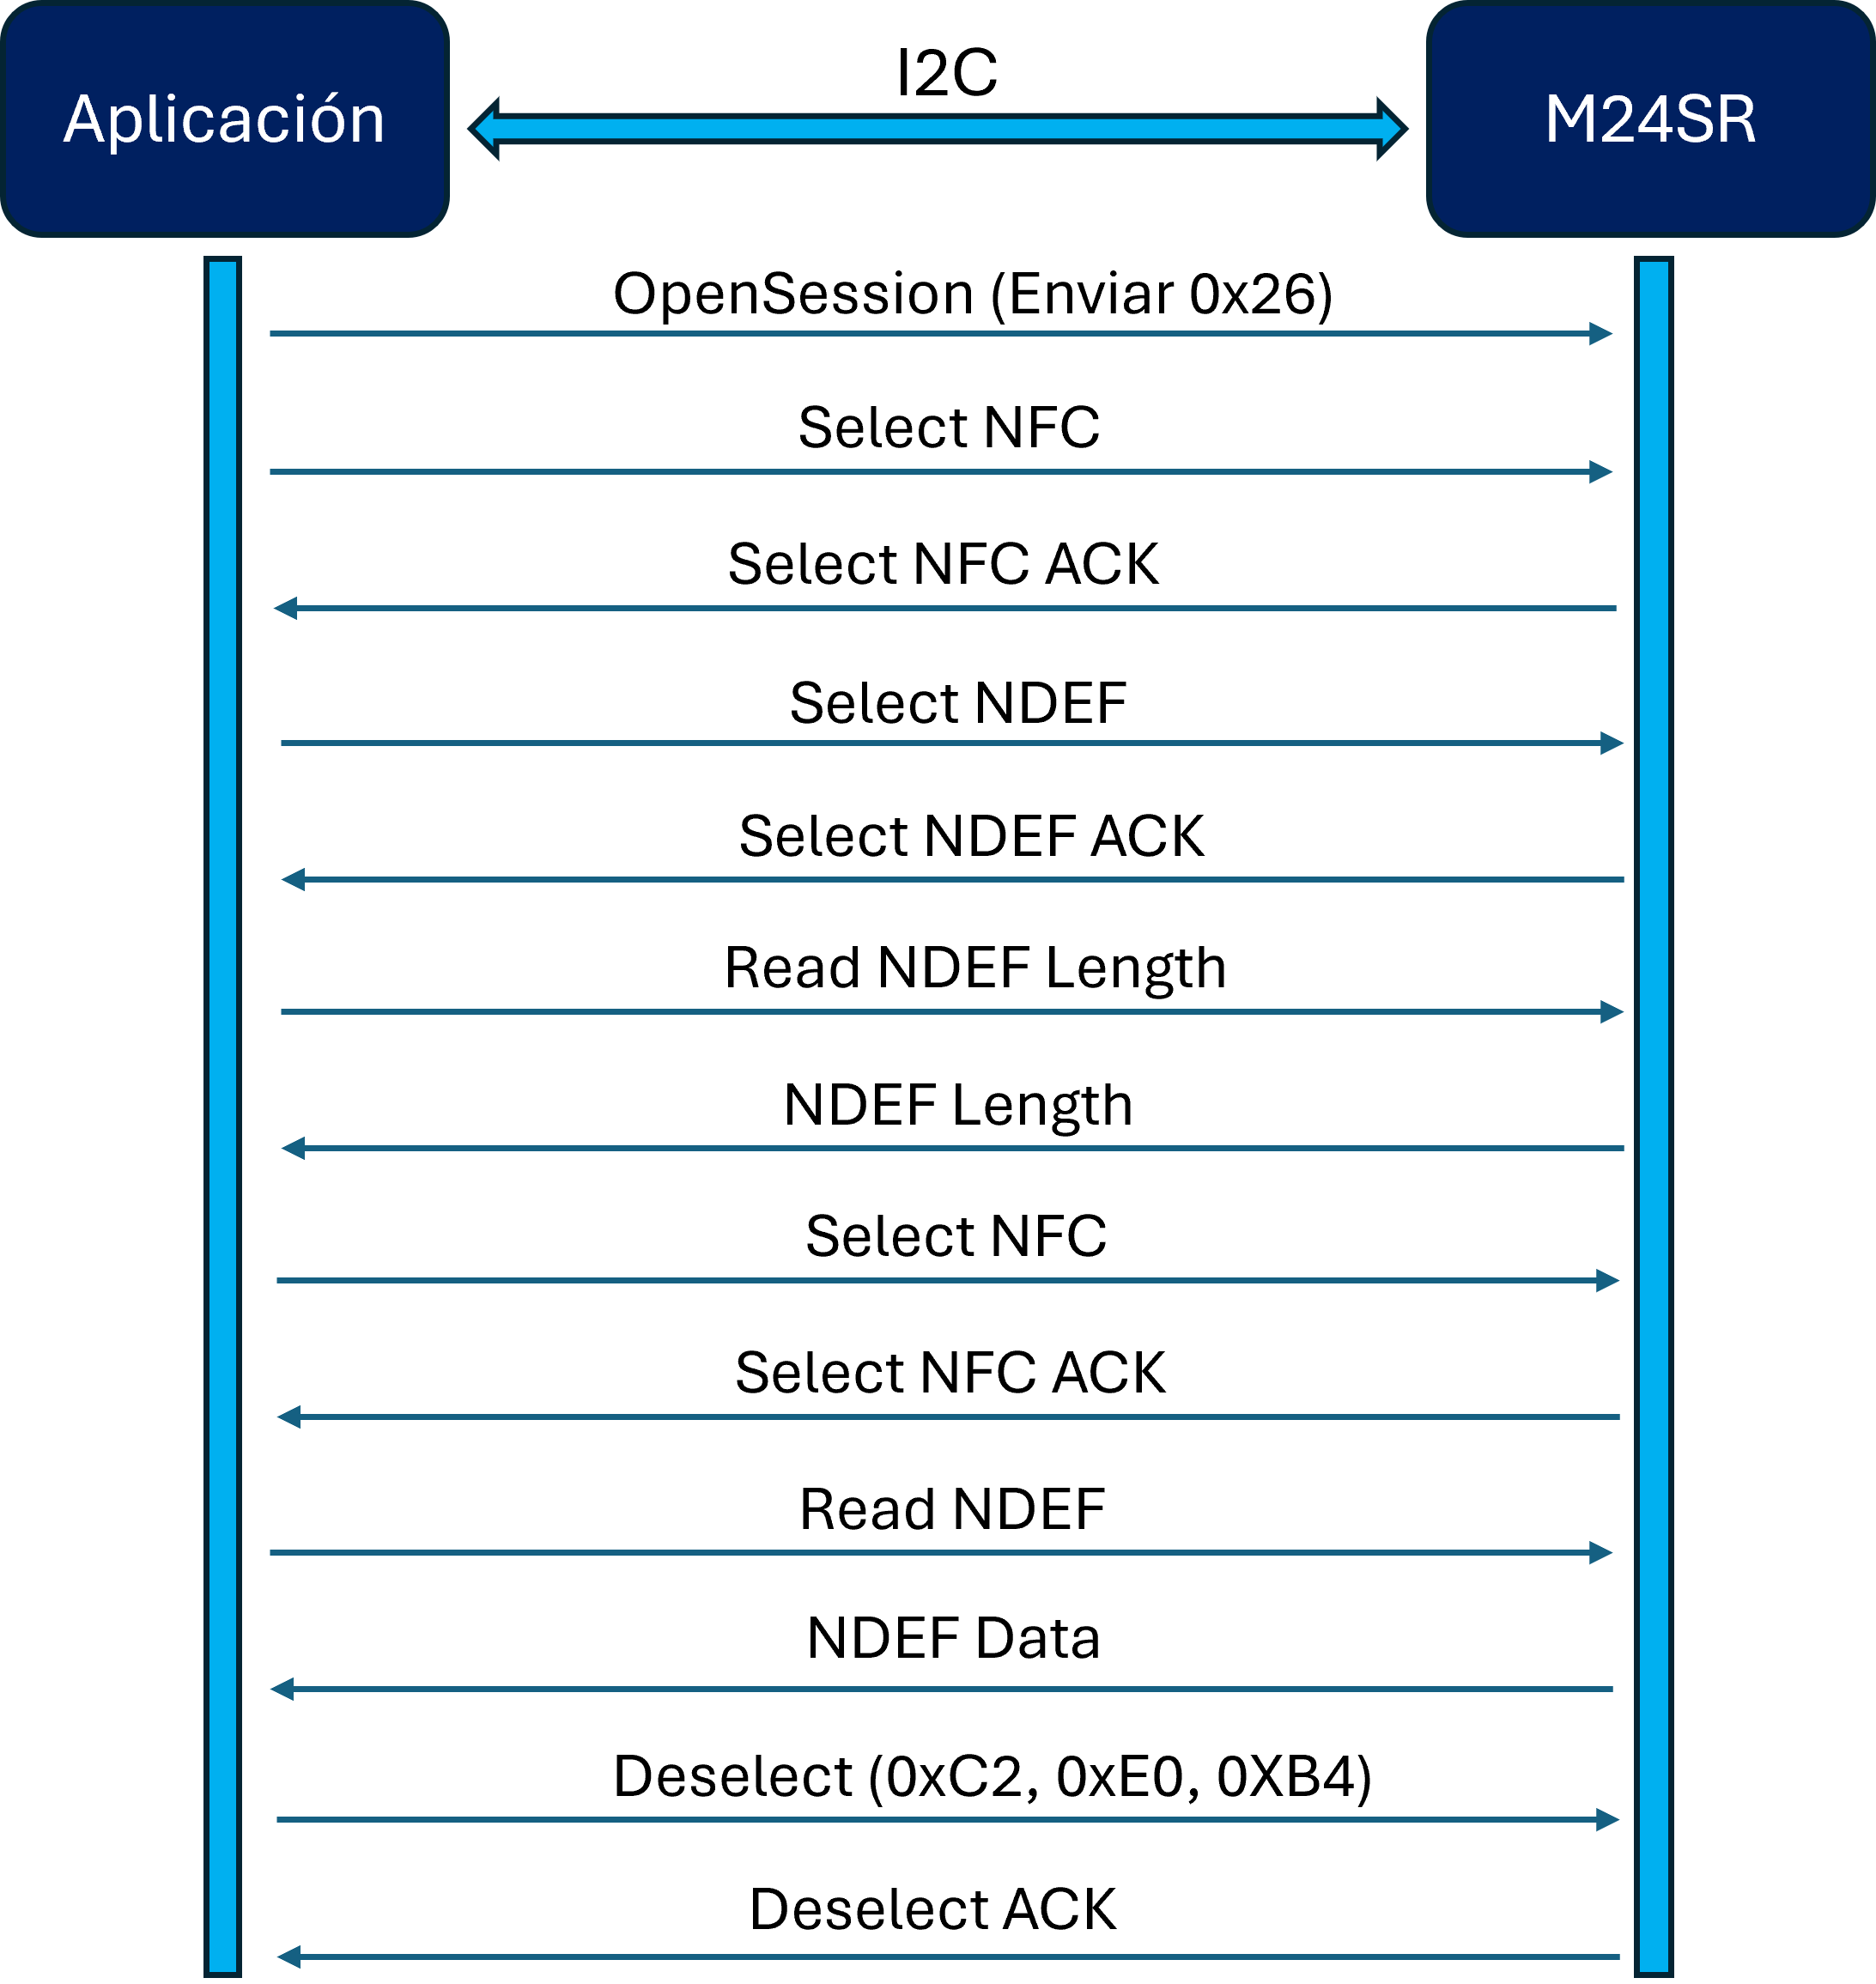
\includegraphics[width=0.5\textwidth]{images/3/3-2/SD/Diagrama.png}
    \caption{Diagrama de flujo de una operación de lectura con el NFC}
    \label{fig:label}
\end{figure}

Todos los bytes para las transferencias los hemos calculado gracias al datasheet del componente M24SR64-Y. Además, antes de enviar el master recieve, hay que esperar por los tiempos de la tarjeta (\texttt{osDelay(5)}).

El módulo también utiliza CRC para la detección de errores en transferencias I2C. Cada byte I2C se calcula utilizando ese algoritmo, y al final de la trama se envían 2 bytes con el valor calculado. Para cacularlo, hemos utilizado la siguiente página web \cite{CalculoCRC}, introduciendo todos los bytes de la trama.

Los mensajes que hemos definido para el NFC están compuestos por una letra ('S' = canción, 'R' = radio) y 4 números (Nº canción o emisora de radio).

Ejemplos: 
	- \texttt{S 0014}: Se quiere escuchar la canción nº 14.
	- \texttt{R 1029}: Se quiere escuchar la emisora 102.9 FM.
Se encarga al inicio de la aplicación, de acceder a la tarjeta uSD para obtener la lista de canciones y la configuración guardada. Cuando se le indica, se encarga de guardar la configuración actual para poder iniciarse en el próximo encendido con la misma configuración. 

Para su desarrollo, primero intentamos utilizar el driver \texttt{SD} de la placa \texttt{STM32F769I-Disco}, la librería \textit{FatFs} \cite{FatFsModuleApplication}\cite{FatFsGenericFAT} y una tarjeta micro-SD.

Hemos decidido almacenar en la tarjeta el siguiente contenido:
- \texttt{songs.txt}: Lista de canciones. Máximo puede haber 25 canciones, de 30 caracteres cada una (29 en Windows debido al salto de línea). 
- \texttt{config.txt}: Configuración del sistema. Valor de las 5 bandas de ecualización y del volumen.


La estructura del código necesario para este proyecto es:
- FatFs:
	- \texttt{ff.c}, \texttt{ff.h}
	- \texttt{ff_gen_drv.c}, \texttt{ff_gen_drv.h}
	- \texttt{diskio.c}, \texttt{diskio.h}
	- \texttt{sd_diskio.c}, \texttt{sd_diskio.h}
- uSD:
	- \texttt{sd.c}, \texttt{sd.h}
	- \texttt{fatfs_storage.c}, \texttt{fatfs_storage.h}

FatFS es un módulo genérico de sistena de archivos FAT/exFAT para pequeños sistemas embebidos. Es independiente de la plataforma en la que se utilice. Está compuesto por las librerías mencionadas en la estructura.

FatFs se utiliza como abstracción sobre el sistema de ficheros Fat. En nuestro nivel de aplicación solo necesitamos llamar a las funciones de fichero \texttt{ff}. Sin embargo, tenemos que crear una clase que permita unir las librerias FatFs (mediante \texttt{diskio.h}) con la implementación hardware de la uSD. Nosotros utilizamos para ello la clase \texttt{sd_diskio}, mediante el Board Support Package (BSP) de la \texttt{STM32F769I-Disco}.

\begin{figure}[h]
    \centering
    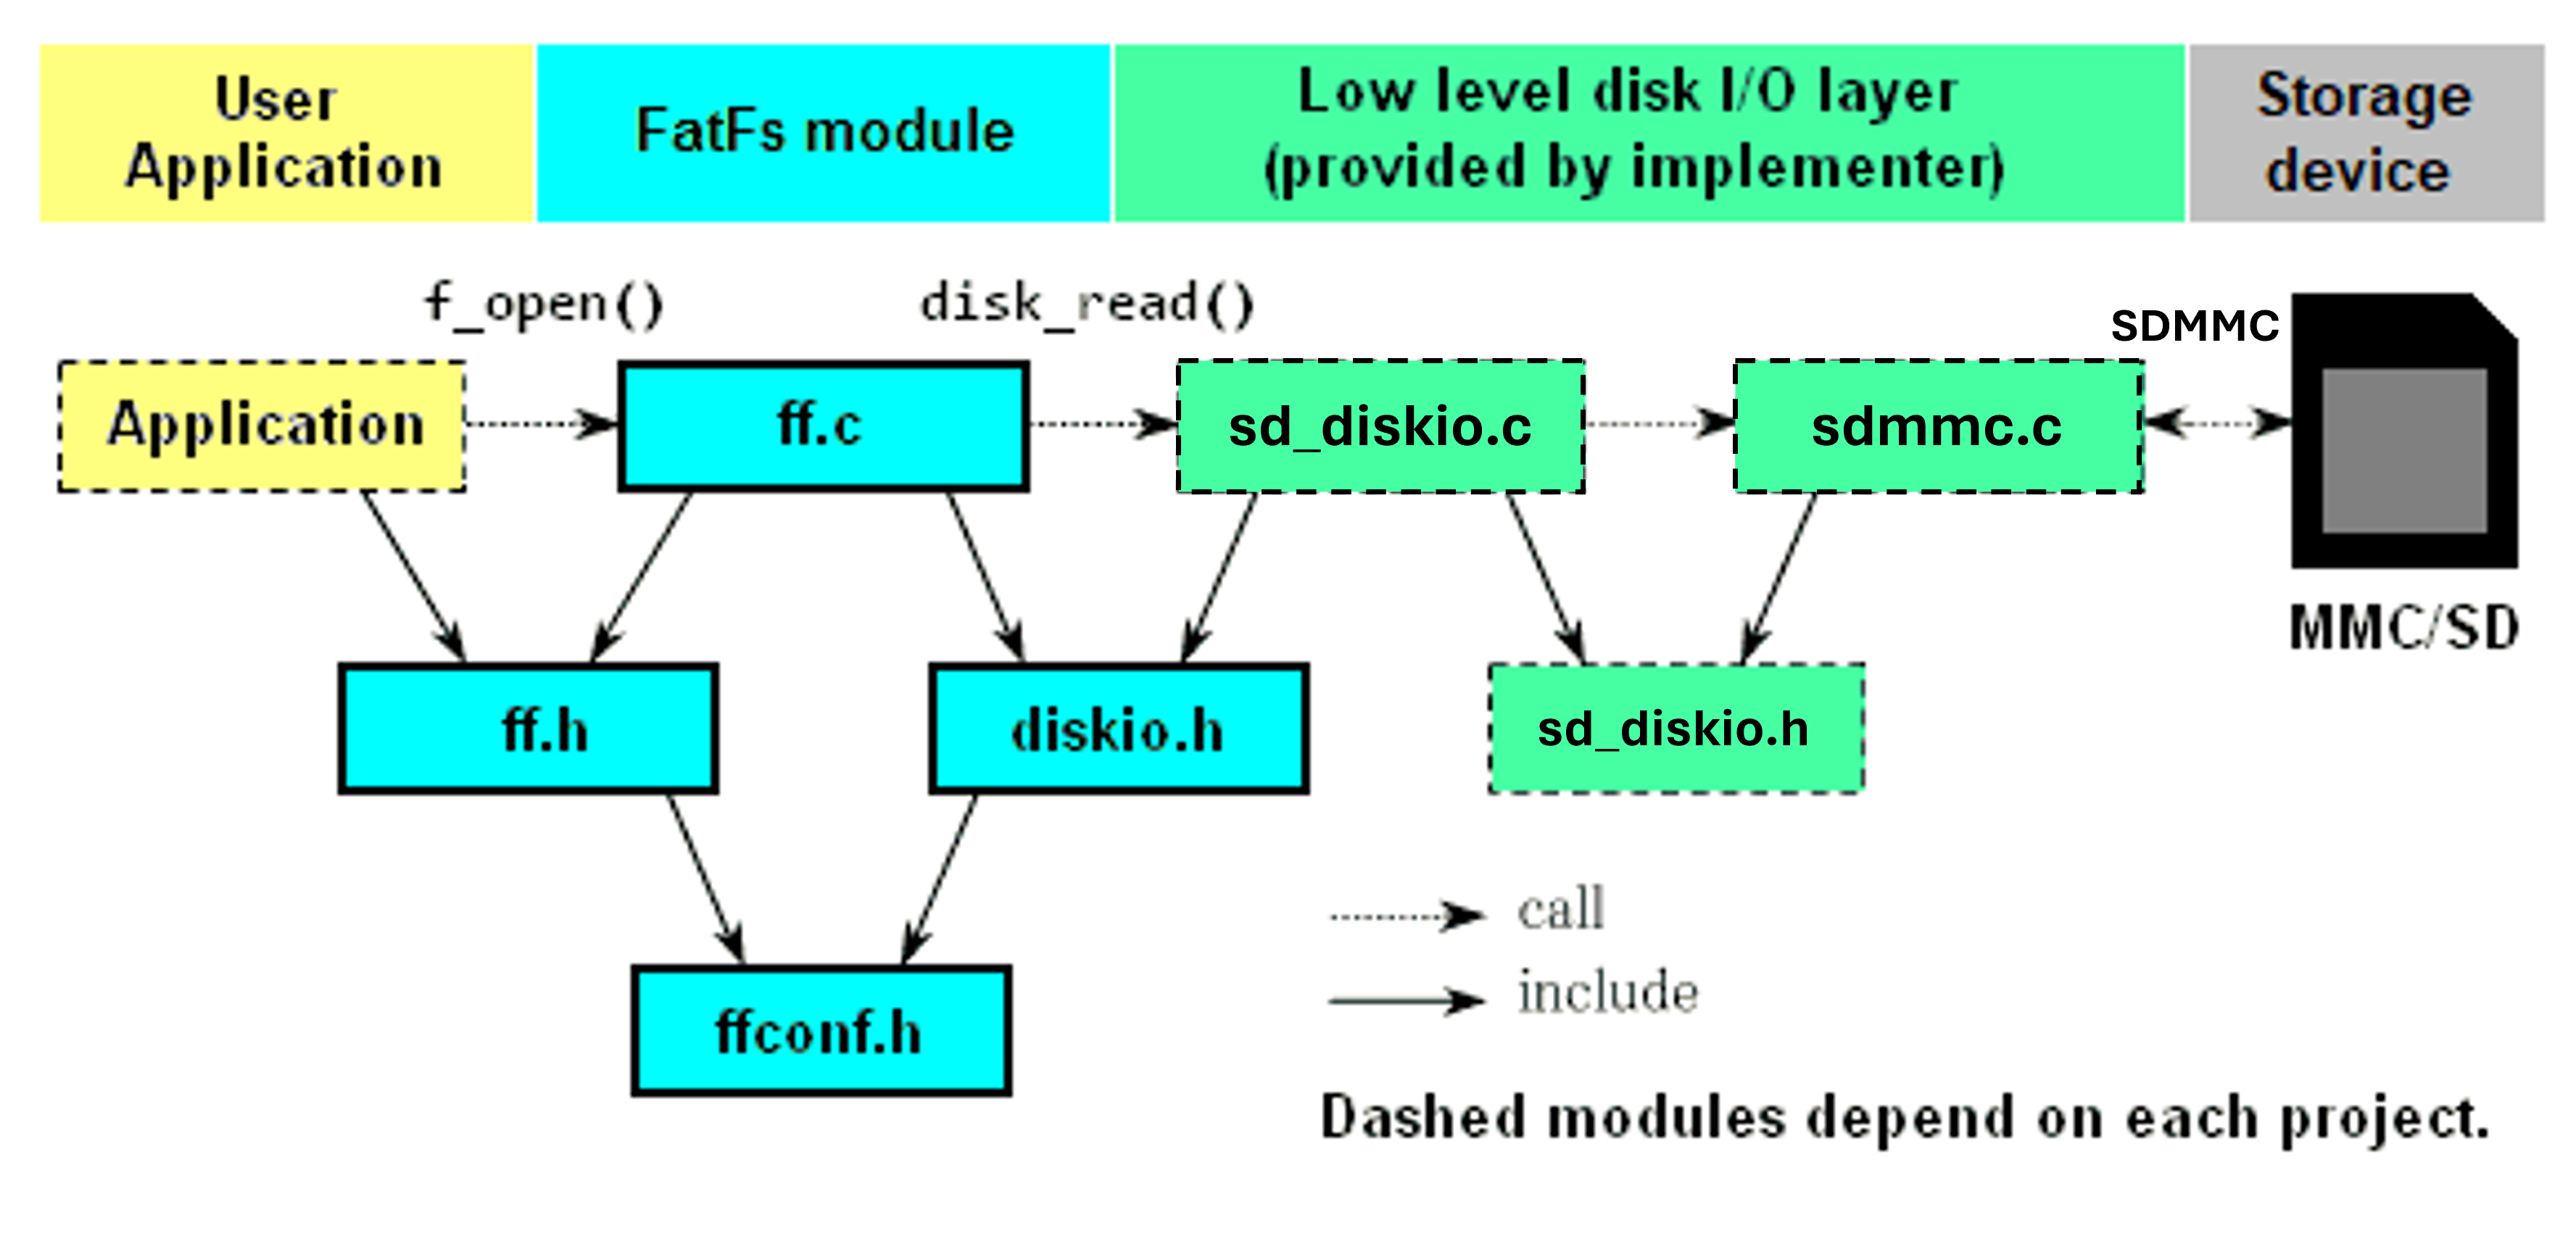
\includegraphics[width=0.5\textwidth]{images/3/3-2/SD/FatFs_1.png}
    \caption{Configuración del sistema implementando FatFs}
    \label{fig:sistema-fatfs}
\end{figure}

Los ficheros \texttt{sd.c} y \texttt{sd.h} se encargan de inicializar la tarjeta, obtener la lista de canciones y la configuración guardada, y de guardar la configuración actual. Esto lo hace utilizando las funciones definidas en \texttt{fatfs_storage.h}. Además, se encarga de revisar que los valores son correctos y están en el rango adecuado. Si no están dentro del rango, los modifica al valor más cercano dentro del rango. También se encarga de adaptar todo lo obtenido a los tipos de variables correctos para la integración del proyecto.

En primer lugar, se inicializa la uSD con la función pública \texttt{Init_SD}. Basicamente se monta la tarjeta y se obtienen el directorio, las canciones (\texttt{Get_Songs}) y la configuración guardada (\texttt{Get_Config}). Toda la información se guarda en punteros a variables del control. Después, cuando se quiere guardar la configuración, se llama a la función pública \texttt{Save_Config}.

Para parsear toda la información lo hacemos de la siguiente manera:

\begin{itemize}
	\item Parseo de la lectura de la configuración: Utilizamos un \texttt{sscanf}.
	\item Parseo de la lectura de las canciones: Utilizamos un algoritmo de copia de cadena de caracteres de triple puntero.
	\item Parseo de la escritura de la configuración: Utilizamos un \texttt{sprintf}.
\end{itemize}

\texttt{fatfs_storage.c} y \texttt{fatfs_storage.h} se encargan de las operaciones de lectura y escritura de los archivos. Esto lo lleva a cabo mediante llamadas a las funciones de las librerías de FatFs. Tiene tres funciones diferentes:

\begin{itemize}
    \item Storage_GetDirectoryBitmapFiles: Se monta la tarjeta con f_mount y se obtiene el directorio de ficheros. El directorio se obtiene llamando a la función de FatFs \texttt{find_first} y después con \texttt{find_next} mientras existan más ficheros. Al final, se cierra el directorio con \texttt{closedir}. (\texttt{f_mount} -> \texttt{f_findfirst} -> \texttt{f_findnext} -> \texttt{f_closedir}).
    \item Storage_OpenReadFile: Se lee un archivo. Primero se abre el archivo, después se lee y finalmente se cierra. (\texttt{f_open} -> \texttt{f_read} -> \texttt{f_close}).
    \item Storage_OpenWriteFile: Se escribe en un archivo. Primero se abre el archivo, después se desplaza el puntero de escritura al principio del fichero .txt y se escribe en él. Finalmente se cierra. (\texttt{f_open} -> \texttt{f_lseek} -> \texttt{f_write} -> \texttt{f_close}).
\end{itemize}

Sin embargo, a la hora de realizar la integración con el resto del proyecto, no funcionaba. La tarjeta llegaba a montarse de manera correcta, pero a la hora de buscar los ficheros, devolvía un \texttt{RXOVER}, que indica que la transferencia de lectura ha sufrido de overflow. 



\subsubsection{Módulo RTC}
El principal objetivo de este módulo es mostrar la hora y la fecha actual en el sistema. Esto se consigue mediante el periférico RTC del propio microcontrolador.

Dicho reloj se ha configurado para que se conecte al oscilador interno LSE, que cuenta con una frecuencia de 32.768kHz. Debido a esta frecuencia, se ha configurado el periférico con unos valores \texttt{AsynchPrediv = 127} y \texttt{SynchPrediv = 255} para obtener un periodo de 1 segundo.

Por otra parte, para obtener la hora actual, se ha optado por utilizar una sincronización con un servidor mediante SNTP.

También se ha configurado el RTC para generar una interrupción mediante una alarma con una frecuencia de 1Hz. En el callback de dicha alarma, se informa a este módulo, mediante una flag, que debe indicar al módulo principal, la fecha y la hora actuales. Dicha comunicación se realiza mediante una cola de mensajes.
\subsubsection{Módulo Radio}
El módulo del Sintonizador FM consiste en un \textit{Thread} que se encarga de gestionar el funcionamiento del propio módulo. La comunicación entre el periférico y el microcontrolador se ha configuradao mediante el \textit{Driver I2C} proporcionado por \textit{CMSIS}.

Cuenta con dos colas de mensajes, una en la que el programa principal introduce los mensajes con los comandos que desea que ejecute el Sintonizador, como sintonizar una frecuencia, hacer un \textit{Seekup} o un \textit{SeekDown}, etc. La otra cola se utiliza para que la radio introduzca mensajes con información sobre las frecuencias sintonizadas. Los mensajes mandados por esta cola son del tipo \textit{MSG\_RADIO}.

También cuenta con un \textit{timer} periódico, con un periodo de medio segundo, que se encarga de leer los registros del sintonizador para comprobar su correcto funcionamiento.

Debido a que nuestro sistema cuenta con dos periféricos que utilizan el protocolo \texttt{I2C}, nos hemos visto obligados a utilizar un módulo de gestión del propio protocolo de comunicación, del cual se hablará en el \autoref{subsec:i2c}.

El comportamiento básico de este módulo consiste en una espera mediante un \textit{osMessageQueueGet} de un mensaje proporcionado por el programa principal. Una vez el mensaje es recibido, es procesado y en función de su contenido, se ejecutará el comando correspondiente. En caso de ser un \textit{SeekUp} o un \textit{SeekDown}, el módulo del sintonizador informará al \textit{Thread} principal para que muestre la frecuencia en la que ha terminado.
\subsection{Módulo MP3}
El módulo del reproductor MP3 consiste en un \textit{Thread} que se encarga de controlar la gestión del propio módulo.

Cuenta con una cola de mensajes en la que el programa principal introduce mensajes con el comando a ejecutar. Algunos de estos comandos son reproducir una cancion, pausar su reproducción, siguiente cancion, etc.

Para gestionar la comunicación entre este módulo y el principal, se ha utilizado la USART6 mediante el \textit{Driver\_USART6} proporcionado por CMSIS. Dicha USART se ha configurado atendiendo a las necesidades del reporductor, modo asíncrono, datos de 8 bits sin paridad, utlizando 1 bit de stop y con una velocidad de 9600 bps.

Este módulo no envía mensajes al programa principal debido a que el reproductor no es capaz de leer informaciónde sus propios registros.

El comportamiento básico de este módulo consiste en una espera mediante un \textit{osMessageQueueGet} de un mensaje proporcionado por el programa principal. Una vez el mensaje es recibido, es procesado y en función de su contenido, se ejecutará el comando correspondiente. Una vez la canción es seleccionada, se realiza otra espera mediante un \textit{osThreadFlagsWait} hasta que la transferencia es completada, en cuyo caso el módulo continua con su funcionamiento.
\subsubsection{Módulo Web}
\label{subsec:modulo-web}
Para la generación de las diferenctes páginas web del servidor y la creación de los diferentes scripts para interactuar con dichas páginas, hemos creados varios archivos con extension \texttt{CGI} como el que se adjunta a continuación:

\begin{lstlisting}[captionpos=b, caption={Ejemplo archivo .CGI}, language=html]
    t       <form action="index.cgi" method="post">
    c i 1       <input type="radio" id="entrada_radio" name="entrada" value="radio" OnClick="submit();" %s>
    t               <label for="entrada_radio" style="font-size: 20px;">Radio</label>
    c i 2       <input type="radio" id="entrada_mp3" name="entrada" value="mp3" OnClick="submit();" %s>
    t               <label for="entrada_mp3" style="font-size: 20px;">MP3</label>
    t       </form>
    t           <br><br>
    t       <form action="index.cgi" method="post">
    c i 3       <input type="radio" id="salida_altavoz" name="salida" value="altavoz" OnClick="submit();" %s>
    t               <label for="salida_altavoz" style="font-size: 20px;">Altavoz</label>
    c i 4       <input type="radio" id="salida_cascos" name="salida" value="cascos" OnClick="submit();" %s>
    t               <label for="salida_cascos" style="font-size: 20px;">Cascos</label>
    t       </form>
    \end{lstlisting}

Como se puede observar, existen dos tipos direfentes de líneas de código, las que empiezan por ``t'' y las que empiezan por ``c''. Las que empiezan por ``t'' son ignoradas por el compilador y no se procesan, en cambio, las que empiezan en  por ``c'' son atendidas y procesadas. A continuación, se comprueba la letra siguiente al espacio, en este caso la ``i'', debido a que nos encontramos en el archivo \textit{index.cgi}. Por último, se obtiene el siguiente carácter a continuación del espacio en blanco y, el propio programa del servidor web, tomará unas medidas u otras dependiendo de dicha letra o número. En todos los casos, se sustituirá el ``\%s'' que encontramos al final de dichas líneas de código por el conjunto de carácteres deseado mediante las función \textit{snprintf()}. A continuación se adjunta un trozo de código del programa principal del servidor web en el que se realiza dicha acción:

\begin{lstlisting}[captionpos=b, caption={Ejemplo procesamiento archivo .CGI}]
	switch(env[0]){
		case 'i':
			// Cases for index
			switch (env[2]){
				case '1':
				// Case for Radio Input
					len = sprintf (buf, &env[4], web_state.entrada == WEB_RADIO ? "checked" :"");
				break;
				case '2':
				// Case for MP3 Input
					len = sprintf (buf, &env[4], web_state.entrada == WEB_MP3 ? "checked" :"");
				break;
				case '3':
				// Case for Altavoz Output
					len = sprintf (buf, &env[4], web_state.salida == WEB_ALTAVOZ ? "checked" :"");
				break;
				case '4':
				// Case for Auriculares Output
					len = sprintf (buf, &env[4], web_state.salida == WEB_AURICULARES ? "checked" :"");
				break;
            }
        break;
    }
\end{lstlisting}

Por otra parte, para enviar los datos desde las páginas al programa principal del servidor, se ha optado por usar fótmularios con el método \textit{post}, los cuales se envían si se pulsa algún botón mediante la función \textit{OnClick="submit()"}.

Por último, vamos a comentar la función utilizada para actualizar periódicamente tanto la fecha y la hora como el consumo medido. Esto se ha realizado mediante una función creada en JavaScript llamada \textit{periodicUpdate()}. A continuación se adjunta dicha función en la página denomianada \textit{index}:

\begin{lstlisting}[captionpos=b, caption={Función updatePeriodic()}]
<script language=JavaScript type="text/javascript" src="xml_http.js"></script>
<script>
    var timeUpdate = new periodicObj("time.cgx", 500);
    function periodicUpdateRTC(){
      updateMultiple(timeUpdate,  plotRTCTime);
      rtc_elTime = setTimeout(periodicUpdateRTC, timeUpdate.period);
    }
    function plotRTCTime(){
      timeVal = document.getElementById("rtcTime").value;
      document.getElementById("rtc").textContent = timeVal;
      consumo = document.getElementById("cons_ref").value;
      jg1.refresh(consumo);
    }
</script>
\end{lstlisting}

Como se puede observar, dicha función consiste en una llamada, cada 500ms, al archivo \textit{time.cgx} de donde se obtienen periódicamente los valores de fecha y hora y de consumo. Cuando dichos valores son obtenido, se actualizan sus valores mostrados en las direfentes páginas web. A continuación se adjunta el código presente en el archivo \textit{time.cgx}, el cual tiene un comportamiento idéntico a los archivos con extension \texttt{.CGI} antes mencionados:

\begin{lstlisting}[captionpos=b, caption={Archivo time.cgx}]
t <form>
t <text>
t <id>rtcTime</id>
c h <value>%02d-%02d-20%02d %02d:%02d:%02d</value>
t </text>
t <text>
t <id>cons_ref</id>
c z <value>%04d</value>
t </text>
t </form>
.
\end{lstlisting}


